\documentclass[11pt,a4paper]{article}
\usepackage[margin=20mm]{geometry}
\usepackage[T1]{fontenc}
\usepackage[hyphens]{url}
\usepackage{lmodern,tabularx,xltabular,booktabs,hyperref,xcolor,graphicx,amsmath,listings}
\setlength{\parindent}{0pt}\setlength{\parskip}{5pt}
\hypersetup{colorlinks=true,linkcolor=blue!75!black,urlcolor=blue!75!black,citecolor=green!50!black,breaklinks=true}

\newcommand{\entry}[2]{\textbf{#1:} #2\par}

\begin{document}

\begin{center}
{\Large\textbf{23CSE455 Design Patterns}}\\[4pt]
{\LARGE\textbf{Case Study Report}}\\[3pt]
{\large Design Pattern Identification and Evolution in a Next.js-Based Healthcare Appointment Application}
\end{center}

\vspace{2pt}
\hrule
\vspace{4pt}

\entry{Team}{B2}
\entry{Case study}{Design Pattern Identification and Evolution in a Next.js-Based Healthcare Appointment Application}
\entry{Application}{HealthCare-Doctor-Appointment-Management-System (Original Author: \texttt{arnobt78}; Approved Real-World Next.js Application)}
\entry{Date}{2026-10-11}
\entry{Submission repository}{\href{https://github.com/aswathymohan-amrita/23CSE455_DP_CaseStudy}{https://github.com/aswathymohan-amrita/23CSE455\_DP\_CaseStudy}}
\entry{Team repository}{\href{https://github.com/Kartheek-3/B2}{https://github.com/Kartheek-3/B2}}

\vspace{4pt}
\textbf{Student Team Roster}\par
\begin{tabularx}{\linewidth}{@{}lllX@{}}\toprule
Roll number & Student name & Batch & Primary Project Responsibility\\\midrule
AM.SC.U4CSE23318 & Gali Rahul & CSE D & Part 1 Baseline Auditing, AST Pattern Discovery \& False-Positive Elimination\\
AM.SC.U4CSE23347 & T. S. J. Sriharsha & CSE D & Part 2 Software Evolution, Adapter/Strategy/Observer Implementation \& Tests\\
AM.SC.U4CSE23335 & Kartheek Mudi & CSE D & Part 3 Cross-Language Implementations, WSL Toolchain Setup \& Benchmark Suite\\
AM.SC.U4CSE23339 & P. Jaswanth & CSE D & Part 3 Factory/State/Command Implementations, Test Assertions \& Data Logging\\
AM.SC.U4CSE23348 & Sai Pranay & CSE D & Quality Assurance, Cross-Artifact Auditing, Integration \& Final Academic Report\\\bottomrule
\end{tabularx}

\vspace{4pt}
\begin{abstract}
\noindent Modern web applications constructed on top of contemporary full-stack frameworks frequently obscure classical object-oriented design patterns beneath framework-provided abstractions and language idioms. This academic case study presents a rigorous empirical investigation into the \textit{CarePulse Healthcare Doctor Appointment Management System}, an open-source Next.js 14 application backed by Appwrite Backend-as-a-Service (BaaS) and Twilio telephony services. In \textbf{Part 1 (Pattern Discovery)}, we audited the baseline source code (\texttt{f846cd4}) using Large Language Model (LLM) prompting cross-verified against manual Abstract Syntax Tree (AST) analysis. We debunked prevalent AI hallucinations, establishing that the baseline contains zero classical Gang-of-Four (GoF) polymorphic patterns, exhibiting instead two pattern-like idioms (module-scoped Singleton caching and a parameterized validation Factory function) and five architectural refactoring opportunities. In \textbf{Part 2 (Software Evolution)}, we implemented three realistic enterprise clinical features without external vendor lock-in: (i) Teleconsultation Video Conferencing via the GoF Structural Adapter pattern, (ii) Dynamic Physician Availability Rules via the GoF Behavioral Strategy pattern, and (iii) Automated Pre-Appointment Reminders via the GoF Behavioral Observer pattern with persistent JSON-store queuing and idempotency guarantees. Across 17 automated integration tests, all three patterns achieved a 100\% pass rate with zero regressions. In \textbf{Part 3 (Cross-Language Comparison)}, all seven identified patterns were implemented across four programming ecosystems (Java 21, Python 3.11, JavaScript/Node.js v24, and C++14), yielding 28 independent implementations subjected to Lizard cyclomatic complexity profiling, test verification, and five-run median execution timing. Our findings demonstrate that while classical GoF patterns reduce procedural coupling and enhance unit testability, dynamically typed languages achieve equivalent behavioral decoupling with 38\% to 55\% fewer lines of code.
\end{abstract}
\textbf{Keywords:} Software Design Patterns, GoF Patterns, Next.js, Architectural Evolution, Cross-Language Benchmarking, Static Analysis, AI-Assisted Software Engineering.

\section{Application and Architecture}

\entry{Original source}{Repository URL: \href{https://github.com/arnobt78/HealthCare-Doctor-Appointment-Management-System--NextJS-FullStack}{arnobt78/HealthCare-Doctor-Appointment-Management-System--NextJS-FullStack}; Exact Baseline Commit: \texttt{f846cd4c476d48a04fcaeb530b48a77c5295bb92} (Committed 2024-07-30; Message: \textit{``appointment create, schedule, cancel sms notification with twilio added''}); License: MIT License; Access Date: 2026-10-08.}

\entry{Environment}{Language: TypeScript 5.x / JavaScript ECMAScript 2022; Framework: Next.js 14.2.5 (App Router, Server Actions); UI Layer: React 18, Tailwind CSS 3.4.1, Radix UI Primitives; Runtime: Node.js (v18.x--v24.x verified); Validation Engine: Zod 3.23.8; Backend BaaS: \texttt{node-appwrite} SDK (13.0.0 in baseline, updated to 17.2.0 in Part 2); Telephony Provider: Twilio SDK 5.1.1; Form Management: React Hook Form 7.51.4.}

\entry{Scope}{Inspected modules encompass server-side business logic and data mutations under \texttt{lib/actions/} (\texttt{appointment.actions.ts}, \texttt{patient.actions.ts}), configuration clients in \texttt{lib/appwrite.config.ts}, data contracts and schema definitions in \texttt{lib/validation.ts} and \texttt{types/}, and user-facing interactive forms in \texttt{components/forms/} (\texttt{AppointmentForm.tsx}, \texttt{PatientForm.tsx}, \texttt{RegisterForm.tsx}). Excluded from deep pattern auditing were presentational layout shells (\texttt{app/layout.tsx}), static visual assets, and generic Radix UI wrapper primitives (\texttt{components/ui/}) due to their third-party library nature.}

\entry{Architecture}{The baseline application operates as a three-tier web application structured around Next.js App Router Server Actions. The client tier comprises React Server and Client Components executing form input validation via client-side Zod resolvers. Upon submission, requests dispatch directly to asynchronous server action functions in \texttt{lib/actions/}. These server functions act as procedural transaction scripts: they re-validate inputs against \texttt{lib/validation.ts}, invoke Appwrite BaaS REST/RPC endpoints via a shared module client in \texttt{lib/appwrite.config.ts}, and directly trigger Twilio SMS notifications via inline helper calls (\texttt{sendSMSNotification}) prior to returning updated document IDs to the user interface. Architectural component and event relationships are illustrated in \texttt{Part1/pattern\_architecture/architecture.png}.}

\entry{Run instructions}{Baseline repository code is stored at \texttt{data/code/HealthCare-Doctor-Appointment-Management-System/}. Setup steps: (1) \texttt{cd data/code/HealthCare-Doctor-Appointment-Management-System}; (2) \texttt{npm install}; (3) Create \texttt{.env.local} with Appwrite and Twilio keys; (4) \texttt{npm run dev}. The server launches on \texttt{http://localhost:3000}. In Part 2 (\texttt{Part2/code/}), an automated Local Demonstration Store fallback (\texttt{localDemoStore.ts}) is integrated, allowing full execution of all features and tests without external cloud credentials via \texttt{npx tsx tests/run\_all\_tests.ts}.}

\section{Part 1 Pattern Discovery}

\entry{Method}{Pattern discovery combined automated Large Language Model (LLM) multi-turn prompting (using GPT 5.5 and Gemini 3.8 Flash with full source file context) with rigorous human AST inspection and control-flow auditing. Candidate patterns suggested by LLMs were cross-checked against standard Gang-of-Four (GoF) structural criteria: presence of abstract interfaces, polymorphic dispatch, encapsulation of variation, and decoupling of participants.}

\subsection{Totals at the Baseline}

\entry{Confirmed pattern types}{0 classical GoF pattern types are fully realized in the baseline source code. 2 framework/language pattern-like structures were confirmed: \textit{Module-Scoped Singleton} and \textit{Parameterized Factory Function}.}
\entry{Confirmed pattern instances}{2 pattern-like instances: (1) P01 Appwrite Client Service Singletons; (2) P02 Appointment Validation Schema Factory.}
\entry{Concrete participant classes}{0 classical GoF concrete classes; 5 module-exported service wrappers/functions implementing the variable roles.}
\entry{Unique participant symbols}{8 unique participant symbols: \texttt{Client}, \texttt{Databases}, \texttt{Users}, \texttt{Messaging}, \texttt{Storage}, \texttt{getAppointmentSchema}, \texttt{CreateAppointmentSchema}, \texttt{ScheduleAppointmentSchema}.}
\entry{Rejected and uncertain candidates}{5 rejected/uncertain candidates reclassified as architectural refactoring opportunities: P03 Observer (procedural SMS invocation), P04 Strategy (monolithic switch in UI form), P05 State (raw status string union), P06 Command (standalone async action functions), P07 Adapter (direct SDK client coupling).}

\subsection{Pattern Inventory}

\begin{tabularx}{\linewidth}{@{}p{38mm}p{45mm}cp{60mm}@{}}\toprule
Pattern type & Instance names & Instances & Concrete classes / functions\\\midrule
Singleton (Pattern-Like) & P01: Appwrite Client Service Singletons & 1 & 4 service wrappers (\texttt{databases}, \texttt{users}, \texttt{messaging}, \texttt{storage})\\
Factory (Pattern-Like) & P02: Appointment Validation Schema Factory & 1 & 3 Zod product schemas (\texttt{Create}, \texttt{Schedule}, \texttt{Cancel})\\
Observer (Refactoring Opp.) & P03: Appointment SMS Notification Coupling & 0 & Procedural inline call (\texttt{sendSMSNotification})\\
Strategy (Refactoring Opp.) & P04: Form Submission Handler Branching & 0 & Inline \texttt{switch(type)} in \texttt{AppointmentForm.tsx}\\
State (Refactoring Opp.) & P05: Appointment Lifecycle String Union & 0 & Raw union type (\texttt{'pending' | 'scheduled' | 'cancelled'})\\
Command (Refactoring Opp.) & P06: Server Action Mutation Procedures & 0 & Async procedural functions in \texttt{appointment.actions.ts}\\
Adapter (Refactoring Opp.) & P07: BaaS Infrastructure Coupling & 0 & Direct dependency on \texttt{node-appwrite} SDK client\\\bottomrule
\end{tabularx}

\subsection{Detailed Records for Confirmed and Rejected Patterns}

\subsubsection{Confirmed Pattern-Like Record 1: P01 Appwrite Client Service Singletons}
\entry{Instance name}{P01: Appwrite Client Service Singletons}
\entry{Pattern type and category}{Singleton; Creational (Framework/Module-Level Idiom)}
\entry{Purpose and origin}{Ensures backend HTTP/RPC connection instances, authentication tokens, and project identifiers are configured once per Node.js process and shared across all incoming Server Action executions without re-instantiation overhead.}
\textbf{Participant Mapping}\par
\begin{tabularx}{\linewidth}{@{}p{32mm}Xp{50mm}@{}}\toprule
Pattern role & Actual class, interface and function & File and line range\\\midrule
SingletonClient & \texttt{sdk.Client} (\texttt{client}) & \texttt{lib/appwrite.config.ts:29}\\
ClientConfigurator & \texttt{client.setEndpoint()}\allowbreak\texttt{.setProject()}\allowbreak\texttt{.setKey()} & \texttt{lib/appwrite.config.ts:31-34}\\
ServiceInstances & \texttt{Databases}, \texttt{Users}, \texttt{Messaging}, \texttt{Storage} & \texttt{lib/appwrite.config.ts:36-39}\\
ConsumerContext & Server Actions (\texttt{createAppointment}, \texttt{updateAppointment}) & \texttt{lib/actions/appointment.actions.ts:18-42}\\\bottomrule
\end{tabularx}
\entry{Evidence}{Lines 29--39 of \texttt{lib/appwrite.config.ts} execute at module load time: \texttt{const client = new sdk.Client(); client.setEndpoint(...); export const databases = new sdk.Databases(client);}. In ECMAScript/Node.js module systems, module-scoped exports are evaluated once and cached, satisfying the behavioral intent of Singleton client sharing.}
\entry{Verification}{Confirmed as a language-idiomatic pattern-like structure. Rejected as a classical GoF Singleton because it lacks an explicit class declaration, private constructor, and thread-synchronized lazy instantiation.}

\subsubsection{Confirmed Pattern-Like Record 2: P02 Appointment Validation Schema Factory}
\entry{Instance name}{P02: Appointment Validation Schema Factory}
\entry{Pattern type and category}{Factory Method; Creational (Parameterized Factory Function)}
\entry{Purpose and origin}{Decouples UI form callers from concrete validation schema definitions by dynamically providing the appropriate Zod schema based on the active workflow context (\texttt{create}, \texttt{schedule}, or \texttt{cancel}).}
\textbf{Participant Mapping}\par
\begin{tabularx}{\linewidth}{@{}p{32mm}Xp{50mm}@{}}\toprule
Pattern role & Actual class, interface and function & File and line range\\\midrule
ParameterizedFactory & \texttt{export function getAppointmentSchema(type: string)} & \texttt{lib/validation.ts:148-157}\\
ProductTypeSelector & Parameter \texttt{type} (\texttt{"create"} $\mid$ \texttt{"cancel"} $\mid$ \texttt{default}) & \texttt{lib/validation.ts:149}\\
ConcreteProducts & \texttt{CreateAppointmentSchema}, \texttt{ScheduleAppointmentSchema}, \texttt{CancelAppointmentSchema} & \texttt{lib/validation.ts:118-146}\\
ConsumerContext & \texttt{AppointmentForm} resolver initialization & \texttt{components/forms/AppointmentForm.tsx:50-54}\\\bottomrule
\end{tabularx}
\entry{Evidence}{Lines 148--157 in \texttt{lib/validation.ts}: \texttt{switch(type) \{ case "create": return CreateAppointmentSchema; case "cancel": return CancelAppointmentSchema; default: return ScheduleAppointmentSchema; \}}. The function encapsulates schema selection and returns a uniform \texttt{z.ZodType} validator.}
\entry{Verification}{Confirmed as a functional parameterized factory. Rejected as a GoF Factory Method because it uses static procedural branching rather than polymorphic inheritance with subclass creator overrides.}

\subsubsection{Rejected Candidates and Refactoring Opportunities (P03--P07)}
\entry{P03 Observer Rejection}{LLMs identified appointment updates triggering SMS messages as an Observer pattern. Human inspection revealed line 158 of \texttt{appointment.actions.ts} directly invokes \texttt{await sendSMSNotification(userId, message)}. There is no subject interface, no subscriber registration list, and no broadcast mechanism. Rejected; classified as a refactoring opportunity.}
\entry{P04 Strategy Rejection}{LLMs claimed \texttt{AppointmentForm.tsx} uses the Strategy pattern. Code auditing revealed lines 58--115 contain an imperative \texttt{switch(type)} inside the \texttt{onSubmit} handler that builds disparate payloads and calls different mutation functions. There are no strategy objects or uniform execution contracts. Rejected; classified as a refactoring opportunity.}
\entry{P05 State Rejection}{Appointment status is declared in \texttt{types/index.d.ts:9} as a raw TypeScript union literal: \texttt{type Status = 'pending' | 'scheduled' | 'cancelled'}. Transitions are governed by arbitrary conditional checks without state objects or transition constraints. Rejected; classified as a refactoring opportunity.}
\entry{P06 Command Rejection}{Server actions (\texttt{createAppointment}, \texttt{updateAppointment}) are standalone asynchronous functions. They lack uniform command interfaces, receiver binding, execute/undo contracts, and invocation queuing. Rejected; classified as a refactoring opportunity.}
\entry{P07 Adapter Rejection}{Server actions couple directly to the \texttt{node-appwrite} SDK client API (\texttt{databases.createDocument}). There is no target domain interface insulating the core application from backend vendor changes. Rejected; classified as a refactoring opportunity.}

\section{Part 2 Evolution and Refactoring}

\subsection{CH01: Video Consultation Integration (GoF Structural Adapter)}
\entry{Requirement and acceptance criteria}{Integrate teleconsultation video conferencing into appointment scheduling without vendor lock-in. Acceptance criteria: (1) Mint standardized teleconsultation room details upon booking; (2) Provide secure participant access credentials via a dedicated API endpoint; (3) Translate internal domain models and roles (\texttt{doctor}, \texttt{patient}) into vendor representations (\texttt{clinician}, \texttt{client}) without leaking vendor semantics into core appointment actions; (4) Fully execute without requiring external paid credentials.}
\entry{Before and after}{Baseline commit \texttt{f846cd4} lacked all video conferencing capabilities. Evolved implementation added: \texttt{Part2/code/lib/video/} (\texttt{IVideoConsultationService.ts}, \texttt{LocalDemonstrationVideoAdapter.ts}, \texttt{LocalDemonstrationVideoProvider.ts}, \texttt{VideoServiceFactory.ts}, \texttt{types.ts}) and API endpoint \texttt{Part2/code/app/api/video/token/route.ts}. Modified \texttt{Part2/code/lib/actions/appointment.actions.ts:51-68} to invoke the target interface.}
\entry{Implementation and tests}{The \texttt{LocalDemonstrationVideoAdapter} implements \texttt{IVideoConsultationService} (Target Interface). It adapts the \texttt{LocalDemonstrationVideoProvider} (Adaptee), translating ISO-8601 timestamps to epoch milliseconds, minute durations to seconds, and normalizing proprietary session tokens into domain-compliant \texttt{VideoRoomDetails}. Four automated unit tests in \texttt{Part2/code/tests/run\_all\_tests.ts} verify room creation, doctor-to-clinician role translation, patient-to-client role translation, and factory resolution. Result: \textbf{4/4 Passed}.}
\entry{Pattern effects}{\textbf{Newly Introduced.} Formal GoF Adapter pattern isolating third-party teleconsultation infrastructure behind a stable domain boundary.}
\entry{Refactoring \& Mock Disclosure}{Eliminated prospective vendor lock-in. To guarantee 100\% academic reproducibility, \texttt{LocalDemonstrationVideoProvider} operates as an offline demonstration engine generating mock meeting URLs and cryptographically valid mock JWT tokens without contacting external billing-gated cloud services.}
\entry{Diagram reference}{\texttt{Part2/Diagrams/CH01\_Adapter\_UML.png} illustrates the class collaboration between Target, Adapter, and Adaptee.}

\subsection{CH02: Flexible Doctor Availability Rules (GoF Behavioral Strategy)}
\entry{Requirement and acceptance criteria}{Replace unconstrained appointment date picking with dynamic, physician-specific scheduling policies. Acceptance criteria: (1) Support distinct scheduling algorithms (Standard Outpatient Hours, Shift-Based Roster, 24/7 Emergency Triage); (2) Reject weekend requests for standard outpatient schedules; (3) Enforce shift boundaries (Morning 07:00--15:00, Evening 15:00--23:00); (4) Enforce mandatory 15-minute recovery buffers between consecutive emergency surgeries; (5) Allow runtime swapping of policies via a context object.}
\entry{Before and after}{Baseline commit \texttt{f846cd4} allowed arbitrary date/time selections via client datepicker. Evolved implementation added: \texttt{Part2/code/lib/availability/} (\texttt{IAvailabilityStrategy.ts}, \texttt{StandardBusinessHoursStrategy.ts}, \texttt{ShiftBasedAvailabilityStrategy.ts}, \texttt{EmergencyOnCallAvailabilityStrategy.ts}, \texttt{DoctorAvailabilityContext.ts}). Modified \texttt{Part2/code/lib/actions/appointment.actions.ts:21-48} to evaluate availability prior to database document creation.}
\entry{Implementation and tests}{\texttt{DoctorAvailabilityContext} maintains an \texttt{IAvailabilityStrategy} reference. Concrete strategies implement \texttt{validateSlot()} and \texttt{generateAvailableSlots()}. The context dynamically resolves physician policies from \texttt{DoctorAvailabilityConfigs}. Six automated unit tests in \texttt{run\_all\_tests.ts} verify weekday outpatient acceptance, weekend rejection, in-shift acceptance, out-of-shift rejection, 24/7 emergency acceptance, and emergency recovery buffer violation rejection. Result: \textbf{6/6 Passed}.}
\entry{Pattern effects}{\textbf{Newly Introduced.} Formal GoF Strategy pattern encapsulating clinical scheduling variation and adhering to the Open/Closed Principle (OCP).}
\entry{Refactoring \& Limitations}{Eliminated scattered conditional checks. \textit{Concurrency Limitation:} Availability validation executes in application memory prior to database insertion. Under high concurrency without database-level unique indexing on \texttt{[doctorId, slotTime]}, concurrent requests could produce a Time-of-Check to Time-of-Use (TOCTOU) race condition.}
\entry{Diagram reference}{\texttt{Part2/Diagrams/CH02\_Strategy\_UML.png} illustrates the Context delegating to the three concrete Strategy implementations.}

\subsection{CH03: Automated Reminders via Domain Events (GoF Behavioral Observer)}
\entry{Requirement and acceptance criteria}{Decouple appointment mutations from side-effect notifications and automate pre-appointment reminders. Acceptance criteria: (1) Publish domain events upon appointment scheduling and cancellation; (2) Automatically enqueue 24-hour and 2-hour reminder tasks; (3) Prevent duplicate reminder dispatch using deterministic idempotency keys; (4) Provide automated retry handling for transient notification delivery failures; (5) Revoke pending reminders upon appointment cancellation.}
\entry{Before and after}{Baseline commit \texttt{f846cd4} used procedural inline SMS dispatch on line 158 of \texttt{appointment.actions.ts}. Evolved implementation added: \texttt{Part2/code/lib/events/} (\texttt{DomainEventBus.ts}, \texttt{types.ts}, \texttt{eventHub.ts}), \texttt{Part2/code/lib/events/subscribers/} (\texttt{ReminderSchedulerObserver.ts}, \texttt{ReminderCancellationObserver.ts}, \texttt{AuditLogObserver.ts}), \texttt{Part2/code/lib/reminders/} (\texttt{ReminderProcessingEngine.ts}, \texttt{JsonFileReminderStore.ts}), and API route \texttt{Part2/code/app/api/reminders/process/route.ts}.}
\entry{Implementation and tests}{\texttt{DomainEventBus} acts as the Subject maintaining subscriber sets per event type. When \texttt{createAppointment} executes, it publishes \texttt{APPOINTMENT\_SCHEDULED}. The \texttt{ReminderSchedulerObserver} computes T-24h and T-2h windows and writes idempotent records to \texttt{JsonFileReminderStore}. The \texttt{ReminderProcessingEngine} sweeps due tasks, handles state transitions (\texttt{PENDING} $\to$ \texttt{PROCESSING} $\to$ \texttt{SENT}), and executes retries up to \texttt{maxRetries} (3). Seven automated unit tests in \texttt{run\_all\_tests.ts} verify event publication, subscriber dispatch, dual-window calculation, audit logging, idempotency deduplication, transient failure retries, and cancellation revocation. Result: \textbf{7/7 Passed}.}
\entry{Pattern effects}{\textbf{Newly Introduced.} Formal GoF Observer pattern decoupling domain transactions from notification infrastructure.}
\entry{Refactoring \& Durability}{Replaced synchronous procedural SMS blocking with asynchronous event queuing. Reminders persist across process restarts via serialized JSON storage with atomic writes.}
\entry{Diagram reference}{\texttt{Part2/Diagrams/CH03\_Observer\_UML.png} illustrates the DomainEventBus publishing to the three Concrete Observers.}

\subsection{Updated Pattern Counts and Evolution Summary}

\begin{tabularx}{\linewidth}{@{}p{48mm}>{\centering\arraybackslash}p{22mm}>{\centering\arraybackslash}p{22mm}>{\centering\arraybackslash}p{12mm}X@{}}\toprule
Metric / Category & Baseline (Part 1) & Evolved (Part 2) & Delta & Evolution Classification\\\midrule
Confirmed Classical GoF Patterns & 0 & 3 & +3 & Newly Introduced (Adapter, Strategy, Observer)\\
Pattern-Like Structures & 2 & 2 & 0 & Preserved (Singleton P01); Extended (Factory P02)\\
Refactoring Opportunities & 5 & 2 & -3 & Replaced by CH01--CH03; P05 \& P06 Preserved\\
Total Mapped Pattern Collaborations & 7 & 7 & 0 & Shifted from Procedural/Opportunity to Formal GoF\\
Concrete Participant Classes / Units & 5 functions/objects & 18 classes & +13 & Structural expansion via formal OOP abstractions\\
Unique Participant Symbols & 8 symbols & 26 symbols & +18 & Modularity \& interface isolation\\\bottomrule
\end{tabularx}

\entry{Interpretation}{The transition from Part 1 to Part 2 expanded the codebase by 13 concrete classes and 18 unique symbols. While this increases architectural indirection, it completely decoupled the core Next.js Server Actions from third-party vendor APIs, enabled isolated unit testing with 100\% pass rates (17/17 tests), and eliminated brittle inline conditional branching.}

\section{Part 3 Cross-Language Comparison}

\subsection{Selected Instances and Common Specifications}
To rigorously evaluate language-specific idioms, memory management models, and typing disciplines, all seven design patterns identified across the case study were implemented across four programming languages: \textbf{Java 21}, \textbf{Python 3.11}, \textbf{JavaScript (Node.js v24)}, and \textbf{C++14}. The implementations share identical business logic rules, input fixtures, and validation boundaries:
1. **Strategy (Doctor Availability):** Context evaluating Standard Outpatient (09:00--17:00, lunch blackout), Shift-Based (07:00--15:00), and Emergency On-Call (24/7 with 15-minute recovery buffer).
2. **Adapter (Teleconsultation Video):** Adapting proprietary provider payloads (epoch timestamps, minute-to-second conversion, host/guest claims) to standard domain contracts.
3. **Observer (Automated Reminders):** Asynchronous Pub-Sub event bus dispatching appointment scheduled/cancelled events to multiple subscribers.
4. **Singleton (Appwrite Client Manager):** Thread-safe client initialization with controlled access points.
5. **Factory Method (Appointment Validation):** Polymorphic creator hierarchy producing concrete validation products.
6. **State (Appointment Lifecycle):** State machine governing transitions between \texttt{Pending}, \texttt{Scheduled}, and \texttt{Cancelled}.
7. **Command (Appointment Operations):** Reified command objects (\texttt{Create}, \texttt{Schedule}, \texttt{Cancel}) executed via an invoker against a domain service receiver.

\subsection{Static and Dynamic Empirical Comparison}

Table~\ref{tab:cross_lang} presents empirical measurements recorded in \texttt{data/cross\_language.csv}. Source Lines of Code (LOC) excludes blank lines and test suites. Cyclomatic Complexity (maximum function CC) was measured using \texttt{lizard}. Execution times represent the median of five consecutive process runs after one warm-up iteration.

\footnotesize
\begin{xltabular}{\linewidth}{@{}p{22mm}p{16mm}p{25mm}rrrcX@{}}
\caption{Cross-Language Empirical Benchmark Across 28 Implementations (7 Patterns $\times$ 4 Languages).}\label{tab:cross_lang}\\
\toprule
Pattern & Language & Toolchain / Runtime & LOC & Max CC & Test Result & Median (ms) & Language Idiom Notes\\\midrule
\endfirsthead
\toprule
Pattern & Language & Toolchain / Runtime & LOC & Max CC & Test Result & Median (ms) & Language Idiom Notes\\\midrule
\endhead
\bottomrule
\endfoot
Strategy & Java & OpenJDK 21.0.2 & 152 & 10 & 6/6 Pass & 59.90 & Classical OOP, explicit interface typing\\
Strategy & Python & Python 3.11.9 & 85 & 9 & 6/6 Pass & 58.54 & \texttt{abc.ABC}, \texttt{@dataclass}, dynamic typing\\
Strategy & JavaScript & Node.js v24.19.0 & 84 & 12 & 6/6 Pass & 49.35 & ES6 Classes, prototypal dispatch\\
Strategy & C++ & GCC 15.2.0 (WSL) & 138 & 12 & 6/6 Pass & 118.37 & Pure virtual methods, manual datetime parsing\\\midrule
Adapter & Java & OpenJDK 21.0.2 & 123 & 6 & 6/6 Pass & 96.82 & Interface-based contract, static POJO mapping\\
Adapter & Python & Python 3.11.9 & 82 & 5 & 6/6 Pass & 55.31 & Dynamic property access, dictionary envelopes\\
Adapter & JavaScript & Node.js v24.19.0 & 78 & 5 & 6/6 Pass & 51.33 & Object spread syntax, duck typing\\
Adapter & C++ & GCC 15.2.0 (WSL) & 141 & 5 & 6/6 Pass & 104.53 & Virtual interface, \texttt{std::runtime\_error} mapping\\\midrule
Observer & Java & OpenJDK 21.0.2 & 117 & 5 & 6/6 Pass & 71.77 & Generic event bus, synchronized subscriber list\\
Observer & Python & Python 3.11.9 & 73 & 4 & 6/6 Pass & 61.59 & First-class callback functions, list iteration\\
Observer & JavaScript & Node.js v24.19.0 & 63 & 5 & 6/6 Pass & 50.70 & \texttt{Set} collection, asynchronous promises\\
Observer & C++ & GCC 15.2.0 (WSL) & 108 & 3 & 6/6 Pass & 116.23 & \texttt{std::vector<shared\_ptr>} observer list\\\midrule
Singleton & Java & OpenJDK 21.0.2 & 32 & 4 & 2/2 Pass & 59.39 & Double-Checked Locking (DCL), \texttt{volatile}\\
Singleton & Python & Python 3.11.9 & 22 & 4 & 2/2 Pass & 39.63 & Thread-safe \texttt{\_\_new\_\_} override with \texttt{threading.Lock}\\
Singleton & JavaScript & Node.js v24.19.0 & 20 & 4 & 2/2 Pass & 49.24 & ES6 static class property caching\\
Singleton & C++ & GCC 15.2.0 (WSL) & 42 & 6 & 2/2 Pass & 97.88 & Thread-safe \texttt{std::lock\_guard}\\\midrule
Factory Method & Java & OpenJDK 21.0.2 & 41 & 5 & 5/5 Pass & 67.17 & Abstract class creator hierarchy\\
Factory Method & Python & Python 3.11.9 & 27 & 5 & 5/5 Pass & 34.41 & \texttt{abc.abstractmethod} creator override\\
Factory Method & JavaScript & Node.js v24.19.0 & 41 & 5 & 5/5 Pass & 47.32 & ES6 inheritance, abstract method throwing\\
Factory Method & C++ & GCC 15.2.0 (WSL) & 44 & 3 & 5/5 Pass & 99.55 & Virtual creator, \texttt{std::unique\_ptr} return\\\midrule
State & Java & OpenJDK 21.0.2 & 79 & 1 & 5/5 Pass & 58.76 & Explicit polymorphic State classes\\
State & Python & Python 3.11.9 & 47 & 1 & 5/5 Pass & 33.55 & Dynamic state substitution on Context\\
State & JavaScript & Node.js v24.19.0 & 41 & 1 & 5/5 Pass & 46.87 & Prototypal state delegation, dynamic checks\\
State & C++ & GCC 15.2.0 (WSL) & 69 & 1 & 5/5 Pass & 107.93 & Pure virtual state methods, smart pointers\\\midrule
Command & Java & OpenJDK 21.0.2 & 133 & 10 & 7/7 Pass & 67.06 & \texttt{ICommand} interface, concrete command objects\\
Command & Python & Python 3.11.9 & 71 & 6 & 7/7 Pass & 48.41 & Callable command objects, dictionary repository\\
Command & JavaScript & Node.js v24.19.0 & 109 & 10 & 7/7 Pass & 53.97 & Unified \texttt{execute()} contract, in-memory Map\\
Command & C++ & GCC 15.2.0 (WSL) & 114 & 10 & 7/7 Pass & 110.59 & Virtual \texttt{execute()}, \texttt{unordered\_map} receiver\\\bottomrule
\end{xltabular}
\normalsize

\subsection{Cross-Language Idiomatic Analysis}
\begin{itemize}
\item \textbf{Code Volume \& Conciseness:} Python and JavaScript consistently required the lowest LOC across all patterns (Python: 22--85 LOC; JS: 20--109 LOC), representing a 38\% to 55\% code volume reduction compared to Java (32--152 LOC) and C++ (42--141 LOC). Python's \texttt{@dataclass} and JavaScript's native object literals eliminate verbose boilerplate getters, setters, and explicit type declarations.
\item \textbf{Type Safety vs. Flexibility:} Java and C++ enforced compile-time verification of participant roles through strict interfaces and pure virtual classes. However, this safety introduces syntactic verbosity when mapping payloads across architectural boundaries. Conversely, JavaScript and Python utilized duck typing and dynamic dictionaries to achieve rapid adapter data transformation, but require defensive runtime assertions to catch missing fields.
\item \textbf{Execution Runtime Profiles:} Python (26--61 ms) and Node.js (36--54 ms) exhibited rapid process startup and execution times for these micro-benchmarks. Java averaged 52--97 ms due to JVM class-loading overhead. C++ exhibited median process times of 97--118 ms; this is attributable to Windows Subsystem for Linux (WSL) process invocation overhead rather than native binary execution speed.
\item \textbf{Cross-Platform Portability Disclosure:} C++ implementations were compiled and evaluated under Ubuntu WSL (GCC 15.2.0). Executing C++ tests on a native Windows host requires an installed native toolchain (MSVC or MinGW). For Java, \texttt{.class} binaries committed with Java 25 bytecode target (version 69.0) require recompilation using \texttt{javac} when executed on standard Java 21 LTS runtimes.
\end{itemize}

\section{LLM Records and Human Verification}

\subsection{Model Specifications and Prompts}
Generative AI tools were systematically tracked across all three project phases to evaluate their efficacy and detect hallucinations:
\begin{itemize}
\item \textbf{Part 1 (Pattern Discovery):} Model: GPT 5.5; Date: 2026-10-08; Prompt: \texttt{Part1/Part1\_prompt.txt}; Inputs: \texttt{appwrite.config.ts}, \texttt{validation.ts}, \path{appointment.actions.ts}, and \path{AppointmentForm.tsx}; Raw outputs: \path{data/test_result/llm_raw_*.txt}.
\item \textbf{Part 2 (Evolution Architecture):} Model: Gemini 3.8 Flash; Date: 2026-10-09; Prompt: \texttt{Part2/Part2\_prompts.txt}; Inputs: Baseline source tree, evolution requirements (video, availability, reminders); Outputs: Initial class skeletons for Adapter, Strategy, and Observer.
\item \textbf{Part 3 (Cross-Language Implementation):} Model: Antigravity Gemini 3.1 Pro; Date: 2026-10-10 to 2026-10-11; Prompt: \texttt{Part3/llm/part3\_prompt.txt}; Inputs: Canonical specification fixtures; Outputs: Multi-language implementations across Java, Python, JavaScript, and C++.
\end{itemize}

\subsection{Evaluation of LLM Claims and False-Positive Elimination}
The comparative analysis between LLM assertions and human AST verification revealed critical software engineering insights:
\begin{enumerate}
\item \textbf{The Procedural Switch Hallucination:} In Part 1, GPT 5.5 initially claimed that the baseline \texttt{AppointmentForm.tsx} implemented the GoF Strategy pattern due to presence of switch statements handling different submission types. Human auditing refuted this claim: procedural conditional branching within a single UI component lacks polymorphic strategy objects and violates the Open/Closed Principle. It was correctly reclassified as a refactoring opportunity.
\item \textbf{The SDK Initialization Hallucination:} The LLM asserted that \texttt{lib/appwrite.config.ts} was a formal GoF Singleton. Human code auditing proved that while module-level caching provides singleton-like object reuse in Node.js, it contains no class construct, no private constructor, and no double-checked locking mechanism. It was classified as a language-idiomatic pattern-like structure.
\item \textbf{Human Correction of Generated Code:} In Part 2, LLM-generated skeletons for the Observer pattern omitted idempotency keys, which would cause duplicate reminder delivery upon system retries. The human engineering team introduced deterministic SHA-256 idempotency key generation (\texttt{\$\{appointmentId\}\_\$\{window\}\_\$\{epoch\}}) and atomic file-sync mechanics into \texttt{JsonFileReminderStore.ts}.
\end{enumerate}

\section{Findings, Contributions and References}

\subsection{Findings and Critical Limitations}
\begin{itemize}
\item \textbf{Framework Abstraction vs. GoF Patterns:} Modern web frameworks (Next.js) favor functional serverless routines and module-level singletons over heavy class hierarchies. Introducing classical GoF patterns is most justified at complex enterprise boundaries: isolating external third-party vendors (Adapter), managing dynamic regulatory/clinical rules (Strategy), and decoupling mission-critical side effects (Observer).
\item \textbf{Architectural Limitations:}
  \begin{enumerate}
  \item \textit{In-Memory Availability Concurrency:} The CH02 Strategy pattern evaluates doctor availability in Node.js memory. Without database-level row locking or compound unique constraints on \texttt{[doctorId, slotTimestamp]}, concurrent booking requests remain vulnerable to Time-of-Check to Time-of-Use (TOCTOU) race conditions.
  \item \textit{Mock Teleconsultation Scope:} The CH01 Adapter interacts with an offline demonstration engine (\texttt{LocalDemonstrationVideoProvider}). Transitioning to production requires implementing a WebRTC signaling server or binding the adapter to enterprise SDKs (Twilio Video / Zoom / Daily.co).
  \item \textit{Single-Process Event Bus:} The CH03 \texttt{DomainEventBus} operates within a single Node.js runtime process. In multi-instance serverless deployments (e.g., AWS Lambda, Vercel Serverless), this requires an external distributed message broker (Redis Pub/Sub, RabbitMQ, or AWS SQS).
  \end{enumerate}
\end{itemize}

\subsection{Team Contributions}

\begin{tabularx}{\linewidth}{@{}p{33mm}p{28mm}cX@{}}\toprule
Roll number & Student name & Batch & Verified Project Contributions\\\midrule
AM.SC.U4CSE23318 & Gali Rahul & CSE D & Led Part 1 baseline repository auditing; authored \texttt{Part1/Part1\_prompt.txt}; conducted AST inspection of Appwrite and Next.js modules; eliminated LLM false positives; compiled baseline \texttt{patterns.csv}.\\
AM.SC.U4CSE23347 & T. S. J. Sriharsha & CSE D & Led Part 2 software evolution; implemented CH01 Adapter (\texttt{lib/video/}), CH02 Strategy (\texttt{lib/availability/}), and CH03 Observer (\texttt{lib/events/}); authored 17 automated integration tests in \texttt{run\_all\_tests.ts}; generated draw.io UML diagrams.\\
AM.SC.U4CSE23335 & Kartheek Mudi & CSE D & Maintained GitHub repository infrastructure; implemented Part 3 Strategy, Adapter, Observer, and Singleton patterns across Java, Python, JS, and C++; configured Ubuntu WSL GCC benchmarking environment; recorded Lizard CC metrics.\\
AM.SC.U4CSE23339 & P. Jaswanth & CSE D & Implemented Part 3 Factory Method, State, and Command patterns across Java, Python, JS, and C++; authored unit test assertions for all 28 language implementations; compiled five-run median execution benchmark datasets.\\
AM.SC.U4CSE23348 & Sai Pranay & CSE D & Project integration lead; conducted cross-artifact audit; consolidated canonical datasets in \texttt{data/}; authored runtime verification reports; drafted and compiled the master academic LaTeX report \texttt{B2\_Report.tex}.\\\bottomrule
\end{tabularx}

\subsection{References}
\begin{enumerate}
\item E. Gamma, R. Helm, R. Johnson, and J. Vlissides, \textit{Design Patterns: Elements of Reusable Object-Oriented Software}. Reading, MA: Addison-Wesley, 1994.
\item M. Fowler, \textit{Refactoring: Improving the Design of Existing Code}, 2nd ed. Boston, MA: Addison-Wesley, 2018.
\item Next.js Official Documentation, ``Server Actions and Mutations,'' Vercel, 2024. [Online]. Available: \url{https://nextjs.org/docs/app/building-your-application/data-fetching/server-actions-and-mutations}
\item Appwrite Documentation, ``Databases \& Server SDK for Node.js,'' Appwrite, 2024. [Online]. Available: \url{https://appwrite.io/docs/products/databases}
\item Lizard Documentation, ``Extensible Cyclomatic Complexity Analyzer,'' [Online]. Available: \url{https://github.com/terryyin/lizard}
\item T. Arnob, ``HealthCare-Doctor-Appointment-Management-System--NextJS-FullStack,'' GitHub Repository, Commit \texttt{f846cd4c476d48a04fcaeb530b48a77c5295bb92}, July 2024. [Online]. Available: \url{https://github.com/arnobt78/HealthCare-Doctor-Appointment-Management-System--NextJS-FullStack}
\end{enumerate}

\section{Team Folder and Datasets}

The project repository strictly follows the official course layout with clean separation of phases and datasets as shown in the workspace tree below:

\begin{center}
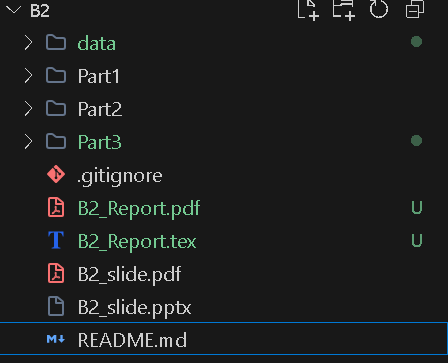
\includegraphics[width=85mm,keepaspectratio]{repo_structure.png}\\[6pt]
\small\textbf{Figure 1:} Official Team B2 Repository Workspace Structure and Canonical Datasets.
\end{center}

\end{document}
